\documentclass{standalone}
\usepackage{tikz}
\usepackage{ctex,siunitx}
\usepackage{tkz-euclide}
\usepackage{amsmath}
\usetikzlibrary{patterns, calc}
\usetikzlibrary {decorations.pathmorphing, decorations.pathreplacing, decorations.shapes,}
\begin{document}
\small
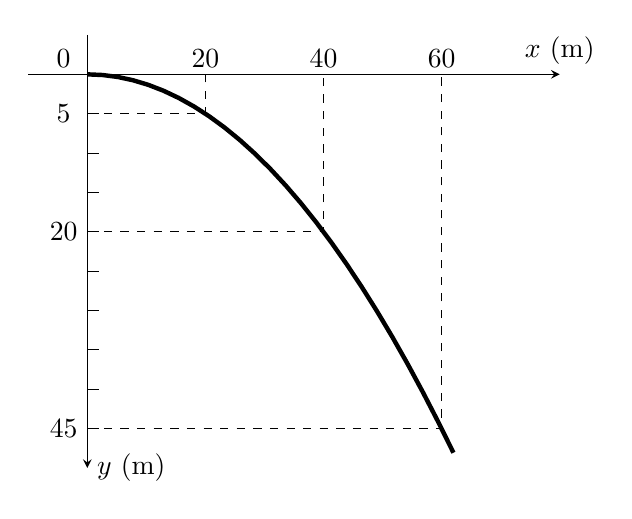
\begin{tikzpicture}[>=stealth, xscale=1.5, yscale=1, domain=0:3.1]
  \draw[->,  thin] (-.5,0)--(4,0)node [above]{$x$ (\unit{m})};
  \draw[->,  thin] (0,.5)--(0,-5)node [right]{$y$ (\unit{m})};
  \foreach \x in {-0.5,-1,-1.5,...,-4.5}
  {
      \draw (0,\x)--(.1,\x);
  }
  \draw[dashed](0,-0.5)--(1,-0.5)--(1,0);    \draw[dashed](0,-2)--(2,-2)--(2,0);    \draw[dashed](0,-4.5)--(3,-4.5)--(3,0);
  \node at (-.2,.2){0};
  \node at (1, .2){20};   \node at (2, .2){40};   \node at (3, .2){60};
  \node at (-.2, -.5){5};   \node at (-.2, -2){20};   \node at (-.2, -4.5){45};
  \draw[ultra thick] plot (\x,-\x*\x/2 ) ;
\end{tikzpicture}
\end{document}